%%%%%%%%%%%%%%%%%%%%%%%%%%%%%%%%%%%%%%%%%%%%%%%%%%%%%%%%%%%%%%%%%%%%%%%%%%%
%
% Template for a LaTex article in English.
%
%%%%%%%%%%%%%%%%%%%%%%%%%%%%%%%%%%%%%%%%%%%%%%%%%%%%%%%%%%%%%%%%%%%%%%%%%%%

\documentclass{article}

% AMS packages:
\usepackage{amsmath, amsthm, amsfonts}
\usepackage{graphicx}
\usepackage{caption}
\usepackage{subcaption}

% Theorems
%-----------------------------------------------------------------
\newtheorem{thm}{Theorem}[section]
\newtheorem{cor}[thm]{Corollary}
\newtheorem{lem}[thm]{Lemma}
\newtheorem{prop}[thm]{Proposition}
\newtheorem{exem}{Example}
\theoremstyle{definition}
\newtheorem{defn}[thm]{Definition}
\theoremstyle{remark}
\newtheorem{rem}[thm]{Remark}
\newcommand{\fim}{ \hfill{\mbox{$\rule{2mm}{2mm}$}}\vskip.6cm }

% Shortcuts.
% One can define new commands to shorten frequently used
% constructions. As an example, this defines the R and Z used
% for the real and integer numbers.
%-----------------------------------------------------------------
\def\RR{\mathbb{R}}
\def\ZZ{\mathbb{Z}}

% Similarly, one can define commands that take arguments. In this
% example we define a command for the absolute value.
% -----------------------------------------------------------------
\newcommand{\abs}[1]{\left\vert#1\right\vert}

% Operators
% New operators must defined as such to have them typeset
% correctly. As an example we define the Jacobian:
% -----------------------------------------------------------------
\DeclareMathOperator{\Jac}{Jac}

%-----------------------------------------------------------------
\title{Further Results on the Prediction of Double Retograde Vaporization Using the Numerical Inversion of Functions from the Plane to the Plane}
\author{Gustavo Barbosa Libotte, Francisco Duarte Moura Neto,\\
L\'{i}via Fl\'{a}via Carletti Jatob\'{a}, Caroline Nascimento Parajara \\ and Gustavo Mendes Platt\\
  \small Polytechnic Institute, Rio de Janeiro State University\\
  \small Rua Bonfim, 25 - Nova Friburgo\\
  \small Brazil
}

\begin{document}
\maketitle

\abstract{This is a simple template for an article written in \LaTeX.}

\section{Introduction}

The double retrograde vaporization phenomenon corresponds to a special shape of the dew-point curve, exhibiting a ``S'' shape (with three dew points) or a double-dome structure (with four dew points). This phenomenon was firstly investigated by \cite{chen_1} and \cite{chen_2} for binary mixtures involving methane + n-butane and methane + n-pentane, under specified temperature. More recently, \cite{raeissi_1} identified a double-dome behavior for the binary mixture ethane + limonene at $T = 307.4$ K and in a narrow range of compositions (close to the pure ethane). Furthermore, \cite{raeissi_2} indicated that the Peng-Robinson equation of state \cite{peng_robinson}, with classical mixing rules, was capable to qualitatively predict this phenomenon.

In the vicinity of the mixture critical point, the robust calculation of dew point pressures (under specified temperature) is a very hard task. Furthermore, some roots of the phase equilibrium problem show very small radius of convergence for Newton-type methods, as indicated by \cite{jnsa}. For this reason, the development of robust frameworks for this kind of problem is extremely relevant. Among several possibilities, we foccus on the robust methodology of the numerical inversion of functions, proposed by \cite{malta}, for functions from
the plane to the plane. This technique \cite{malta} proposes --- considering a restrict set of functions --- the generation of the critical curves in the mathematical 
sense\footnote{The term ``critical''  assumes two meanings in this work: in the mathematical sense, a critical point of a function
 is a nonregular point (where the jacobian matrix is non-invertible); in the thermodynamic sense, the critical point is that where we cannot distinguish between the properties of the phases.}, the construction of a bank of solved points (to be used as 
 with good initial estimates for the solution) and, finally, the inversion of the desired points (calculation of all pre-images of a such image).

As far as we can know, the first application of the methodology  of numerical inversion of two-variable functions in a chemical engineering problem was presented by \cite{canadian}, in the prediction of the azeotropic behavior in systems with double azeotropes.

More recenlty, \cite{ireme} presented some initial results regarding the application of the methodology proposed by \cite{malta} in the prediction of double retrograde vaporization phenomenon in the system ethane + limonene. However, a few relevant aspects were not considered there and we discuss them in this work. Among these aspects, we mention: (i) the influence of the system temperature in the critical curves, and (ii) the analysis of the behavior of inversions near the critical image (where the number of pre-images --- solutions of the system --- change). Furthermore, one of the objectives of this work is to provide a mathematical view of this challenging nonlinear algebraic system, which can be useful in the development of numerical tools for solving high-pressure phase equilibrium problems. As pointed previously, the solution of this kind of nonlinear system with typical root-finding algorithms (such as Newton's methods) is not a trivial task, even when using more sophisticated numerical tools \cite{jnsa}.

Table \ref{tab:roots_double_dome} presents the compositions and pressures for the dew point calculation in the system ethane + limonene at $T = 307.4$ K and $y_1 = 0.998966$, where the ``double-dome'' structure appears, with four dew point pressures (and compositions of the liquid phase). We note, considering the data presented in Table \ref{tab:roots_double_dome}, that one root corresponds to a low pressure root (Root 1) and the othersare high pressure roots (which are close to each other). From the point of view of the calculation techniques -- using classical numerical methods, such as Newton-Raphson methods -- we are interested in robust methodologies capable to find all roots, but mainly with some features to find in a robust way the high pressure roots.

We must mention that the composition of vapor phase is arbitrarily chosen, in order to produce the thermodynamic phenomenon.

\begin{table}[http!]
	\begin{center}
	\begin{tabular}{ccc} \hline \small
Root & $x_1$ & $P$ (kPa) \\
\hline
1 & 0.1567 & 619.26 \\
2 & 0.9829 & 4859.46 \\
3 & 0.9918 & 4931.22 \\
4 & 0.9979 & 5007.25 \\
	\hline
	\end{tabular}
	\caption{ {\small Dew point compositions and pressures for $T = 307.4$ K and $y_1 = 0.998966$.}}\label{tab:roots_double_dome}
	\end{center}
\end{table}

We will use the same numbering to the roots (1, 2, 3 and 4) even for some modified nonlinear problems (without physical significance).

We also tested the dew point calculation at $T = 304.5$ K and $y_1 = 0.99945$, where a ``S'' shape dew curve appears, with three physical roots. The roots are detached in Table \ref{tab:roots_S}.

\begin{table}[http!]
	\begin{center}
	\begin{tabular}{ccc} \hline \small
Root & $x_1$ & $P$ (kPa) \\
\hline
1 & 0.3064 & 1209.36 \\
2 & 0.8442 & 3900.98 \\
3 & 0.9917 & 4671.36 \\
	\hline
	\end{tabular}
	\caption{ {\small Dew point compositions and pressures for $T = 304.5$ K and $y_1 = 0.99945$.}}\label{tab:roots_S}
	\end{center}
\end{table}

\begin{figure}
	\begin{center}
		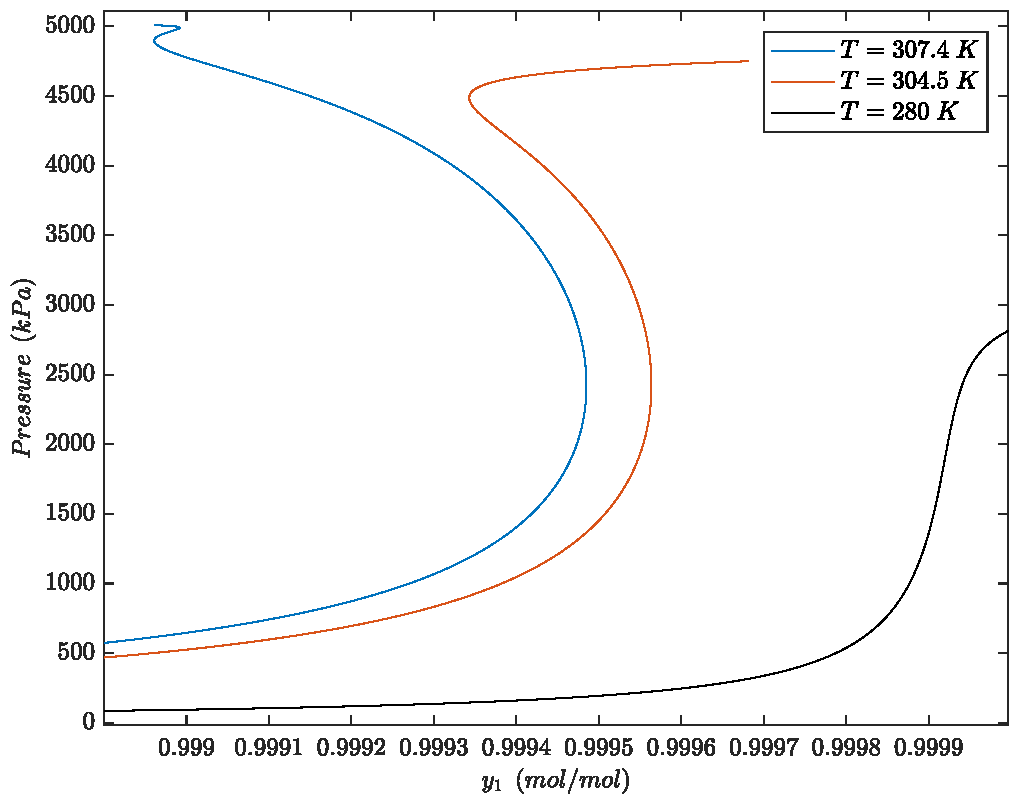
\includegraphics[scale=0.50]{curvas_ponto_orvalho.pdf}
		\caption{Dew point curves for the system ethane + limonene at several temperatures.}\label{fig:dew_point_curve}
	\end{center}
\end{figure}


\section{Models and Methodology}

\subsection{Thermodynamic models and problem formulation}

All the phase equilibrium calculations, as well as the critical point curves (in the thermodynamic sense), will be conducted for the Peng-Robinson equation of state with classical mixing rules and null binary interaction parameters. Critical properties and acentric factors of pure components can be found, for instance, in\cite{ireme}.

For a binary mixture, the phase equilibrium problem can be formulated as:
\begin{eqnarray}
\hat{\phi}_i^L x_i = \hat{\phi}_i^V y_i \hspace{0.1in} i = 1,2
\end{eqnarray}
In the last equation $\hat{\phi}$ represents the fugacity coefficient for component $i$ (using the Peng-Robinson model), $x_i$ is the molar fraction in the liquid phase, $y_i$ represents the vapor phase. The superscripts $L$ and $V$ refer to the liquid and vapor phases, respectively.

Using $x_2 = 1 - x_1$ and $y_2 = 1 - y_1$, the nonlinear algebraic problem (in the plane) is then:
\begin{eqnarray}
\hat{\phi}_1^L x_1 = \hat{\phi}_1^V y_1 \\
\hat{\phi}_2^L (1-x_1) = \hat{\phi}_2^V (1-y_2)
\end{eqnarray}

The vector of unknowns, considering the specification of temperature and vapor molar fractions, is $p = (x_1,P)$. Each residue of the nonlinear equations will be referred as $f_i$, since $F = (f_1,f_2)$.

The nonlinear algebraic system can be re-stated as:
\begin{equation}
F(p) = q,
\end{equation}
where $p$ is a point in the domain and $q$ is a point in the image (range) of $F$. Ordinarily, we are interested to solve $F(p) = (0,0)$ (where $q=(0,0)$ represents the null vector in the euclidean plane).

\subsection{TO BE DELETED - a few ideas on the inversion of 
functions}
To understand the methodology of inversion of functions to solve nonlinear systems of equations, we first consider a simple 1D example.
\begin{exem} 
\begin{em}
Let $F(p)=3p^3-p$. By examining the graph of $F$ it is possible to 
check that the equation for $q$,
\begin{eqnarray*}
F(p)=q, \ \ \text{that is}, \ 3p^3-p=q\ ,
\end{eqnarray*}
has three possibilities as far as the number of solutions, $\eta(q)$,
is concerned,
\begin{eqnarray*}
\eta(q)= \left\{ 
\begin{array}{rl}
1 , & \text{if } q< -2/9\\
2, & \text{if } q= -2/9\\
3 , & \text{if }  -2/9< q  < 2/9 \\
2 , & \text{if } q= 2/9\\
1 , & \text{if } q> 2/9\\
\end{array}
\right.
\end{eqnarray*}
One way to determine the transition points where 
 the number of solutions change
is to look at the image of the critical points. The critical points
(where the derivative is not invertible) satisfy
\begin{eqnarray*}
F'(p)=9p^2-1 = 0, \ \text{that is } p=\pm 1/3\ .
\end{eqnarray*}
Therefore, the transition points are $F(\pm 1/3)=\mp 2/9$. 

Now, the range of $F$ is partitioned in five subsets, 
$\mathbb{R}= R_1\cup T_2\cup R_3 \cup T_4 \cup R_5$, 
\begin{eqnarray*}
\text{transitional sets:}&& T_2=\{-\frac{2}{9}\}, 
\ T_4= \{\frac{2}{9}\}\ ,
\\
 \text{non-transitional sets:} && R_1=]-\infty,-\frac{2}{9}[\ , \ 
 R_3 = ]-\frac{2}{9},\frac{2}{9}[\ , \ R_5=]\frac{2}{9},+\infty[\ .
\end{eqnarray*}
The overall strategy for solving the equation $F(p)=q$ is to 
decompose the range of $F$ in its transitional and non-transitional sets, have 
a bank of solved points with representatives more or less covering
the non-trasitional sets, and to solve the system with the 
bank of solved points as initial guesses.
\end{em}
\fim
\end{exem}

Similarly, with functions from the plane to the plane, 
$F:\mathbb{R}^2\rightarrow \mathbb{R}^2$, satisfying certain
technical regularity requirements, \cite{malta}, one defines the 
critical curves, where the jacobian $JF$ is not invertible,
\begin{eqnarray*}
{\cal C}= \{p\in \mathbb{R}^2 \mid \det(JF|_q)=0\}\ ,
\end{eqnarray*}
and the image of ${\cal C}$, 
${\cal T}=F({\cal C})=\{q=F(p), \text{ for all } p \in {\cal C}\}$, 
the critical image, which defines the curves in the range of $F$ 
delimiting
regions where
transitions on the number of pre-images may occur. 

One of the drawbacks to the application of the theory presented in 
\cite{malta} to problems coming from applications 
that involve the solution of nonlinear $2\times 2$ systems of equations
is not so much that it applies only to a collection of ``regular''
functions, but that the functions have to be defined 
in all points in the plane. In this case, 
the theory then gives a fairly good amount
of information on the solutions of the nonlinear system of equations.
In applications usually, however,  the domain of a function has to
satisfy some 
restrictions due, for instance, to the lack of physical significance
of certain values, or due to existence of singularities, 
which breaks the theory presented in \cite{malta}, but preserves
the overall methodology that they discuss. We 
illustrate some aspects of this issue in the next example.
\begin{exem}
\begin{em}
Let 
$F(p)= -\frac{1}{p+1/2}\frac{1}{p-1/2}(p+\frac{1}{4})(p-\frac{1}{4})$,
and consider the nonlinear equation $F(p)=q$ for given $q$. A simple
examination of the graph of $ F$ shows that the number of solutions
as a function of $q$ is
\begin{eqnarray*}
\eta(q) = \left\{ \begin{array}{lr} 
2, & \text{if } q< -1 \\
0, & \text{if } -1 \leq q < -1/4\\
1, & \text{if } q=-1/4 \\
2, & \text{if } q> -1/4
\end{array}
\right. \ .
\end{eqnarray*}
Again we have the range of $F$ partitioned in regions,
\begin{eqnarray*}
\text{non-transitional sets:}&& R_1=]-\infty,1[\ , R_4=]-1/4,+\infty[\ , 
\\
\text{transitional set:} &&T_3=\{-1/4 \} \ ,
\\
\text{mixed set:} && M_2=[-1,-1/4[ \ .
\end{eqnarray*}

The only critical point, $F'(p)=\frac{3p/8}{(p^2-1/4)^2}=0$, is 0,
and the critical image $F(0)=-1/4$. This is a transitional set, 
however, we are not able to determine the mixed set from this 
calculation. 
\end{em}
\fim
\end{exem}

\subsection{A brief description for some features of the numerical inversion of functions from the plane to the plane}

\section{Numerical Results}

The methodology of numerical inversion of two-variable functions, adapted from \cite{malta} which considered the special case of function from the plane to the plane,
 was employed in this phase equilibrium calculation by \cite{ireme}. In this sense, all details regarding the production of the bank of solved points and the numerical steps of the inversion process are detailed by \cite{ireme}. Here, we will focuses on some aspects not addressed by \cite{ireme}, mainly with regard
 to the quantity of pre-images in  limit-situations (for instance, when we approached to the critical image). Furthermore, we will present the thermodynamic calculation of the critical points for the binary mixture ethane + limonene for the entire range of compositions.
 
\subsection{Thermodynamic critical point calculations}

In this subsection we present the critical curve for the mixture ethane + limonene for the entire range of compositions. As reported previously, the term ``critical curve'' can exhibit two different meanings: the mathematical sense (points where the jacobian is 
singular) and the thermodynamic sense. Here we  deal
 with thermodynamic critical points, and  we use the approach of Heidemman and Khalil \cite{heidemman}, with a double-loop structure in temperature-molar volume, for the critical point calculation.

Figure \ref{fig:critical_thermo} illustrates the critical curve, in the temperature-pressure plane, for the mixture at hand. We observe a continuous and unique curve connecting the two pure components. Thus, this system can be classified as Type I, accordingly to the classification of binary mixtures of Van Konynenburg and Scott \cite{classif}.

\begin{figure}
	\begin{center}
		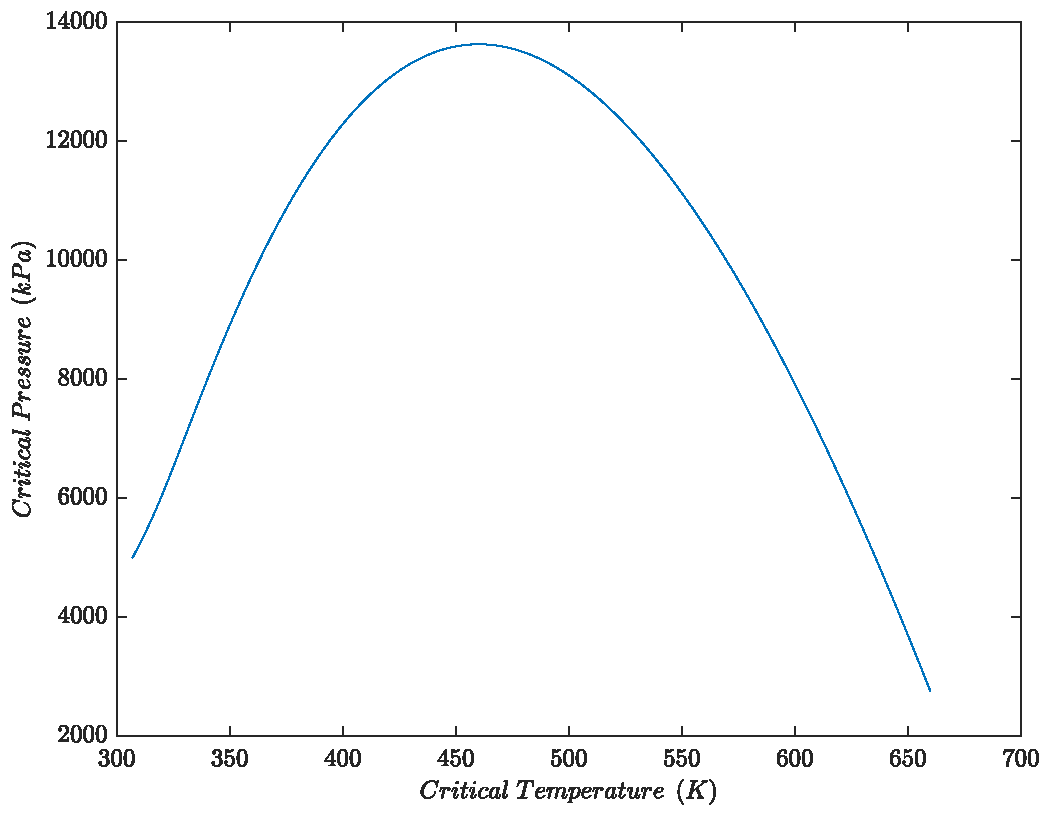
\includegraphics[scale=0.50]{temperatura_pressao.pdf}
		\caption{The thermodynamic critical curve in the system ethane + limonene.}\label{fig:critical_thermo}
	\end{center}
\end{figure}

\subsection{Results at $T$ = 307.4 K and $y_1 = 0.998966$}

\subsubsection{An in-depth examination of the critical curves}

As pointed out previously, the initial results regarding the application of the numerical inversion of functions to the prediction of double retrograde behavior was presented by \cite{ireme}. In that work they investigated some basic features of the critical curves. Here, we present a deeper analysis of the critical curves in this system.

Clearly, we note that --- in the highlighted region --- the critical curves exhibit one self-intersection, as represented in Figure \ref{fig:sinais}. Furthermore, the two critical curves show a ``quasi-tangent'' point (or a meeting point).

\begin{figure}
	\begin{center}
		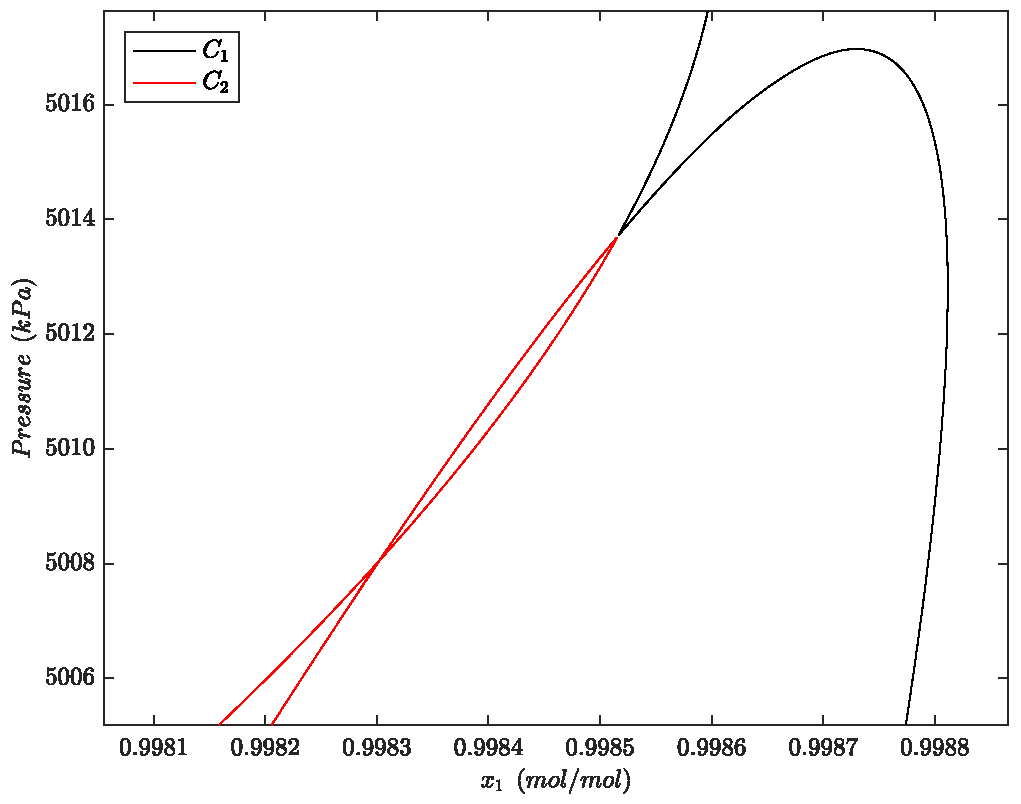
\includegraphics[scale=0.50]{curvas_criticas_dominio_new.pdf}
		\caption{A detailed view of the critical curves.}\label{fig:sinais}
	\end{center}
\end{figure}
 
An amplification of the region in the neighborhood of the ``quasi-tangent'' point, using a color pattern (in order to clarify the relationship between domain and image) is presented in Figure \ref{fig:domain_image}.

\begin{figure}
\centering
\begin{subfigure}{.5\textwidth}
  \centering
  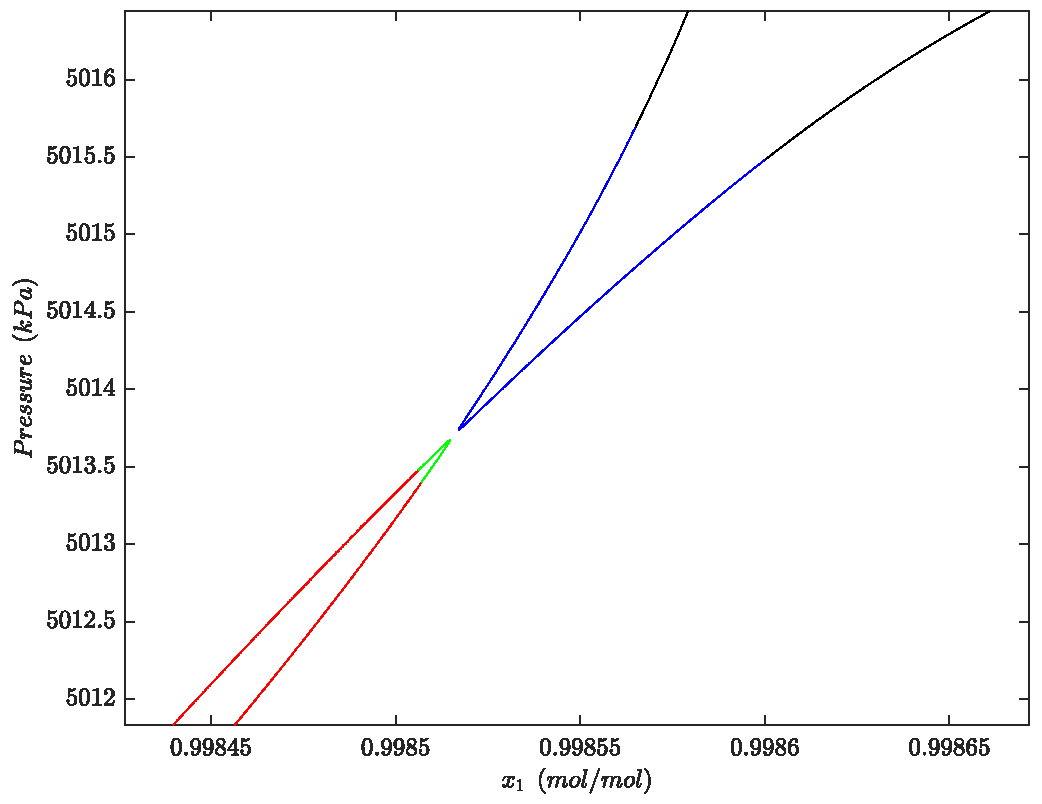
\includegraphics[width=.9\linewidth]{bicos_dominio}
  \caption{Domain}
  \label{fig:sub1}
\end{subfigure}%
\begin{subfigure}{.5\textwidth}
  \centering
  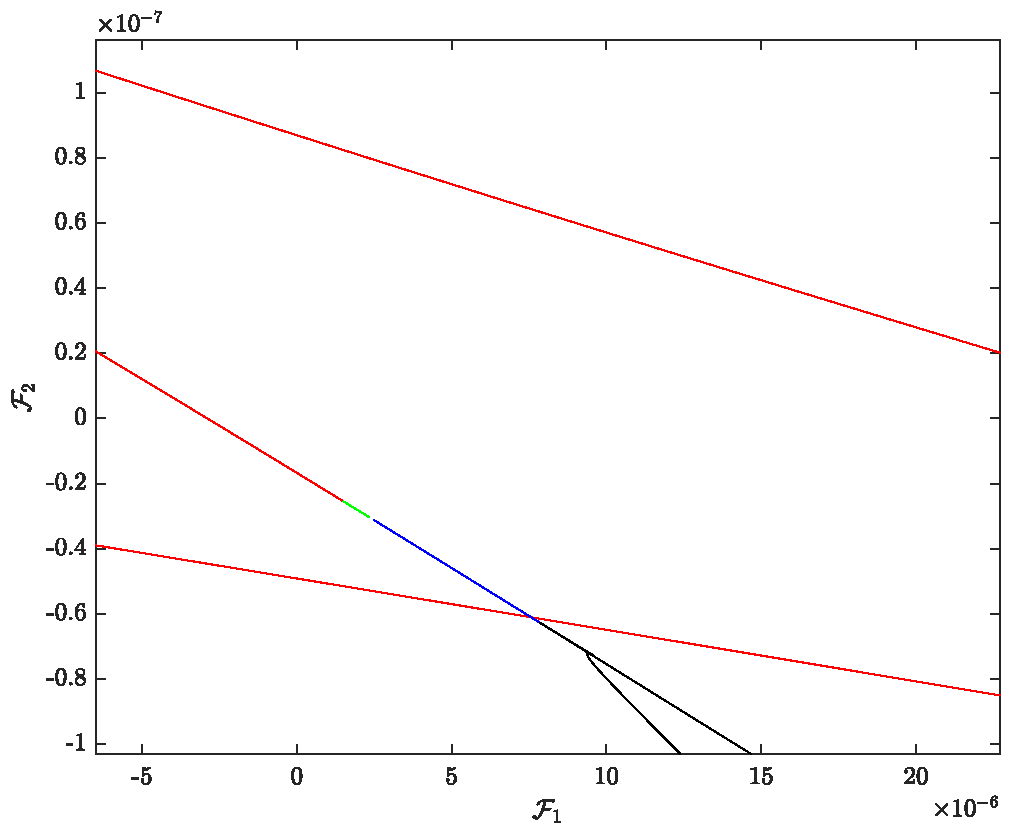
\includegraphics[width=.9\linewidth]{bicos_imagem}
  \caption{Image}
  \label{fig:sub2}
\end{subfigure}
\caption{Amplification of the interest region of the critical curve and the critical image.}
\label{fig:domain_image}
\end{figure}

\subsubsection{Inversion Process -- Approaching to the critical image}

Figure \ref{fig:points_image} presents the sequence of points inverted in the image, beginning at $q = \left(0,0\right)$ and ending close to the critical image (moving to the right side of the image). The squares in the figure are the bank of solved points. The inversion process is then applied, producing the pre-images of the inverted points, in the domain. In this situation, four pre-images are observed (in accordance with the number of solutions of the original nonlinear problem). Obviously, these solutions are not roots of the original problem, since we have $q = (0,0)$ for the physical nonlinear problem. On the other hand, as pointed previously, we will maintain the same numbering of the roots (1, 2, 3 and 4).

The sequence of inverted points -- in the domain -- for Roots 3 and 4 (high pressure roots) is represented by Figure \ref{fig:points_domain_3_4}. The final point inverted is detailed in the zoom (the blue circles). Clearly, we are facing a degeneration process: the number of roots will decay from four to two, since these pre-images tend to the critical curve.

Figures \ref{fig:points_domain_1} and \ref{fig:points_domain_2} contain the sequence of inverted points regarding the Roots 1 and 2, respectively. In these cases, the inverted points are not close to the critical curves.

\begin{figure}
	\begin{center}
		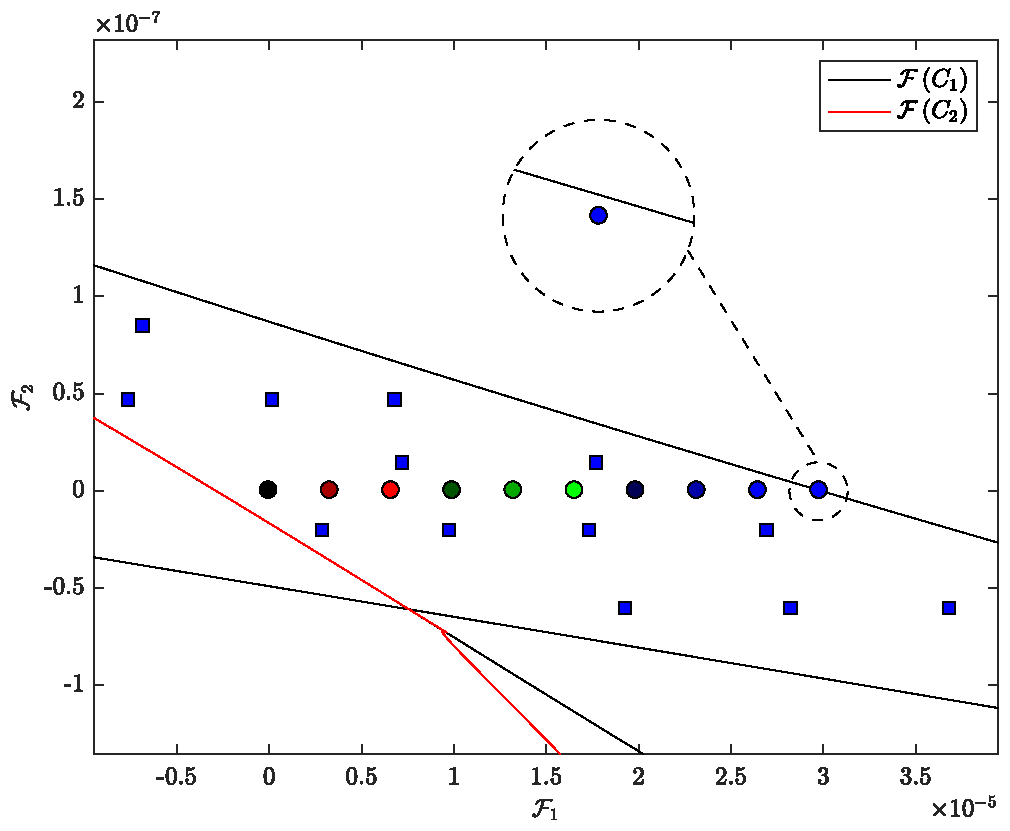
\includegraphics[scale=0.50]{sequencia_pontos_imagem.pdf}
		\caption{Sequence of inverted points (image).}\label{fig:points_image}
	\end{center}
\end{figure}

\begin{figure}
	\begin{center}
		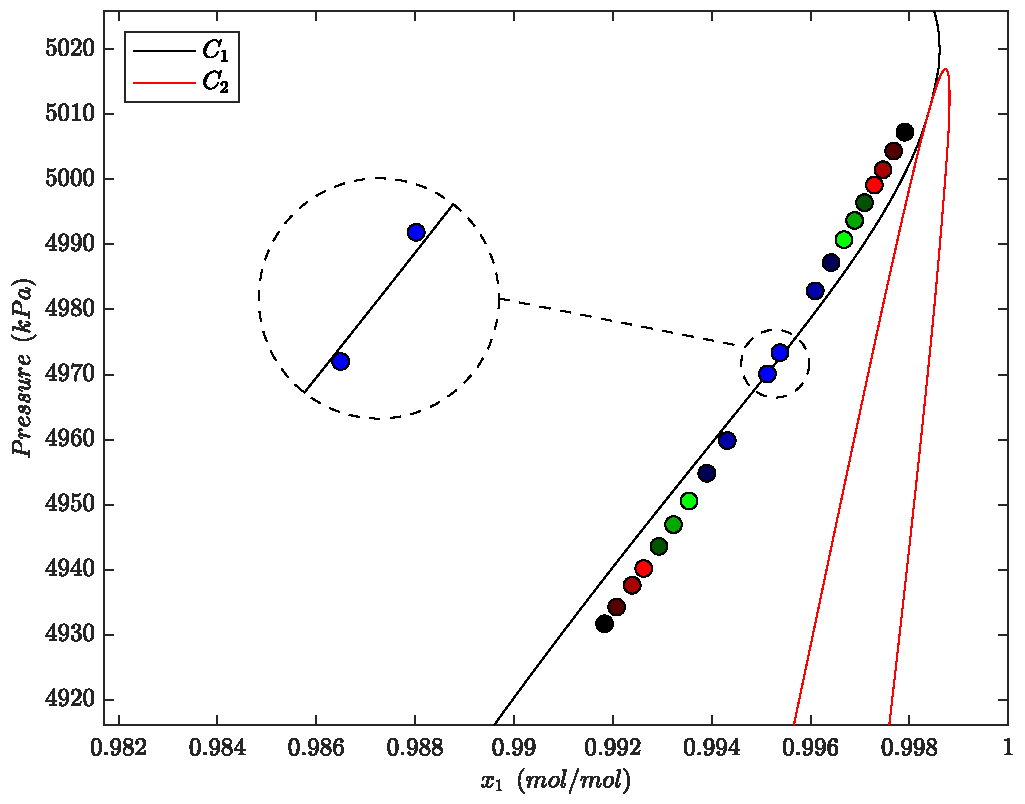
\includegraphics[scale=0.50]{sequencia_pontos_dominio.pdf}
		\caption{Sequences of inverted points (domain), Roots 3 and 4.}\label{fig:points_domain_3_4}
	\end{center}
\end{figure}

\begin{figure}
	\begin{center}
		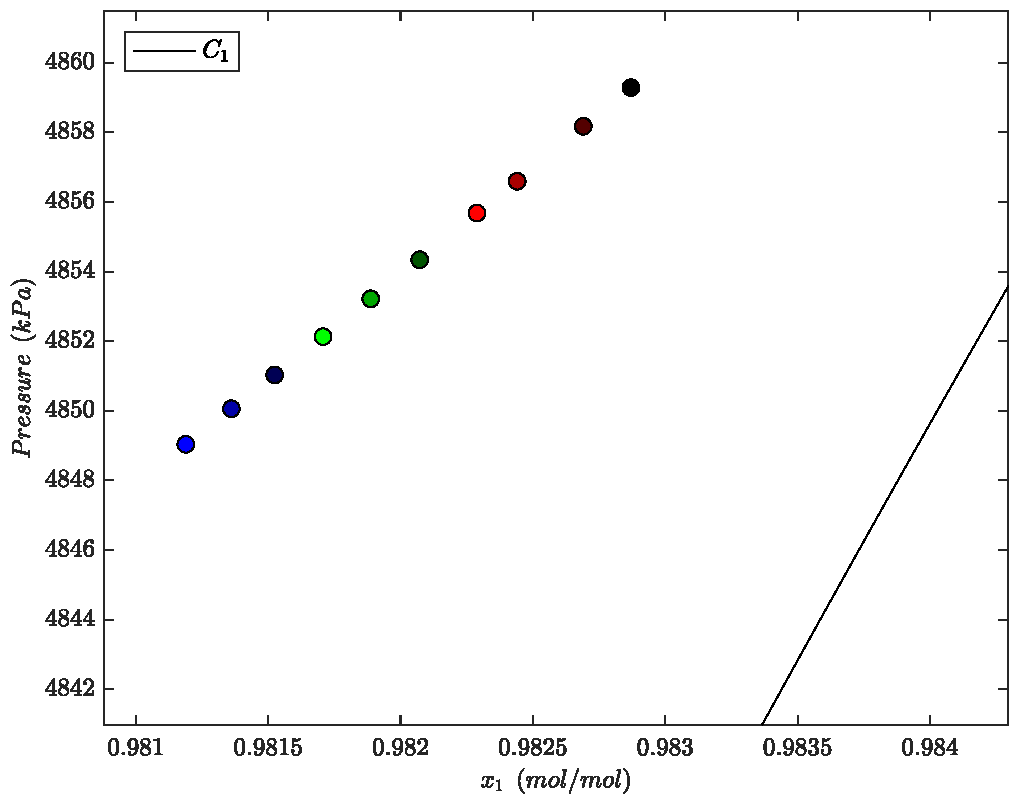
\includegraphics[scale=0.50]{sequencia_pontos_dominio_2.pdf}
		\caption{Sequence of inverted points (domain), Root 2.}\label{fig:points_domain_2}
	\end{center}
\end{figure}

\begin{figure}
	\begin{center}
		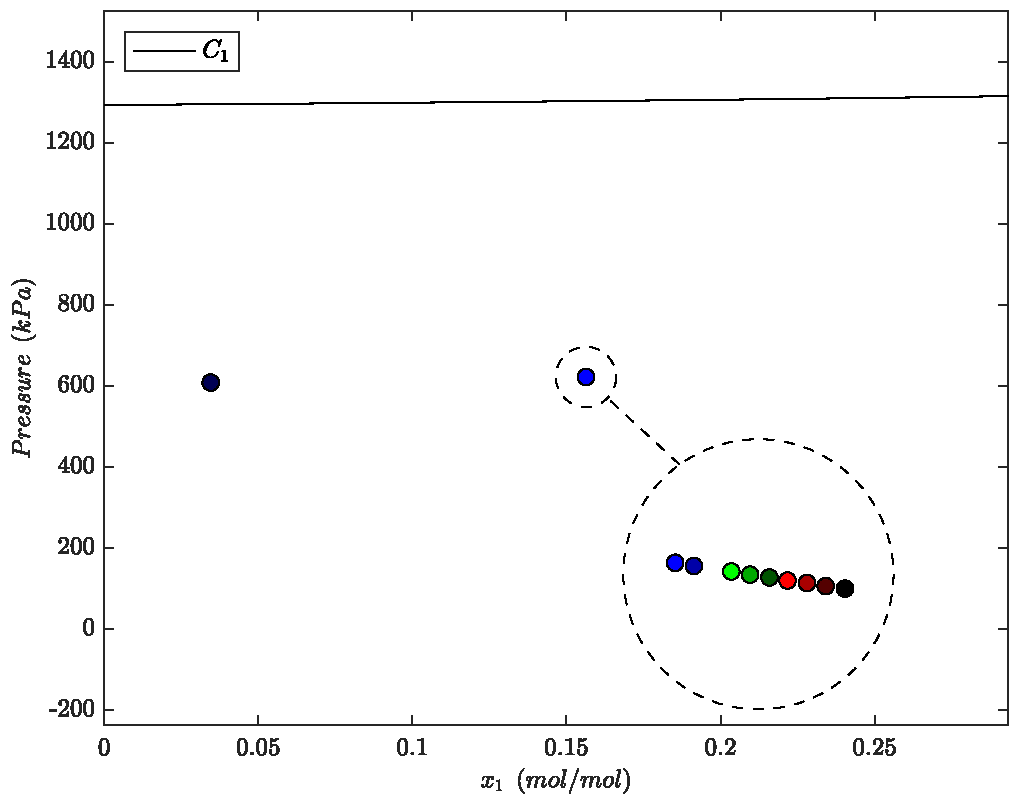
\includegraphics[scale=0.50]{sequencia_pontos_dominio_3.pdf}
		\caption{Sequence of inverted points (domain), Root 1.}\label{fig:points_domain_1}
	\end{center}
\end{figure}

The inversion process will be detailed for the point close to the critical image. Figure \ref{fig:L_path_image} indicates the ``L'' path in the image. Again, the square is a point in the bank of solved points and the desired point is represented by a circle.

\begin{figure}
	\begin{center}
		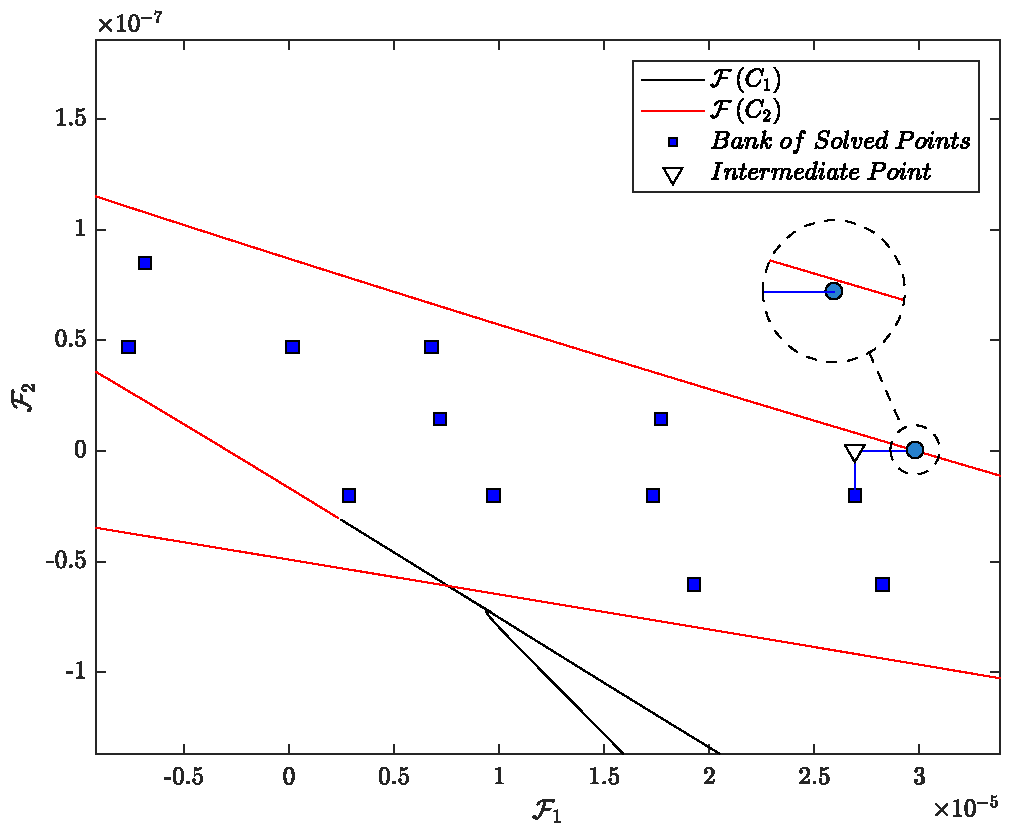
\includegraphics[scale=0.50]{caminho_L_degeneracao_imagem_new.pdf}
		\caption{The ``L'' path in the image.}\label{fig:L_path_image}
	\end{center}
\end{figure}

The paths in the domain are detached in Figure \ref{fig:L_path_domain}. We can note that the ``L'' paths were deformed and are virtually straight lines. Once again, the degeneration process is clearly indicated and the critical curve has a fold at this point.

\begin{figure}
	\begin{center}
		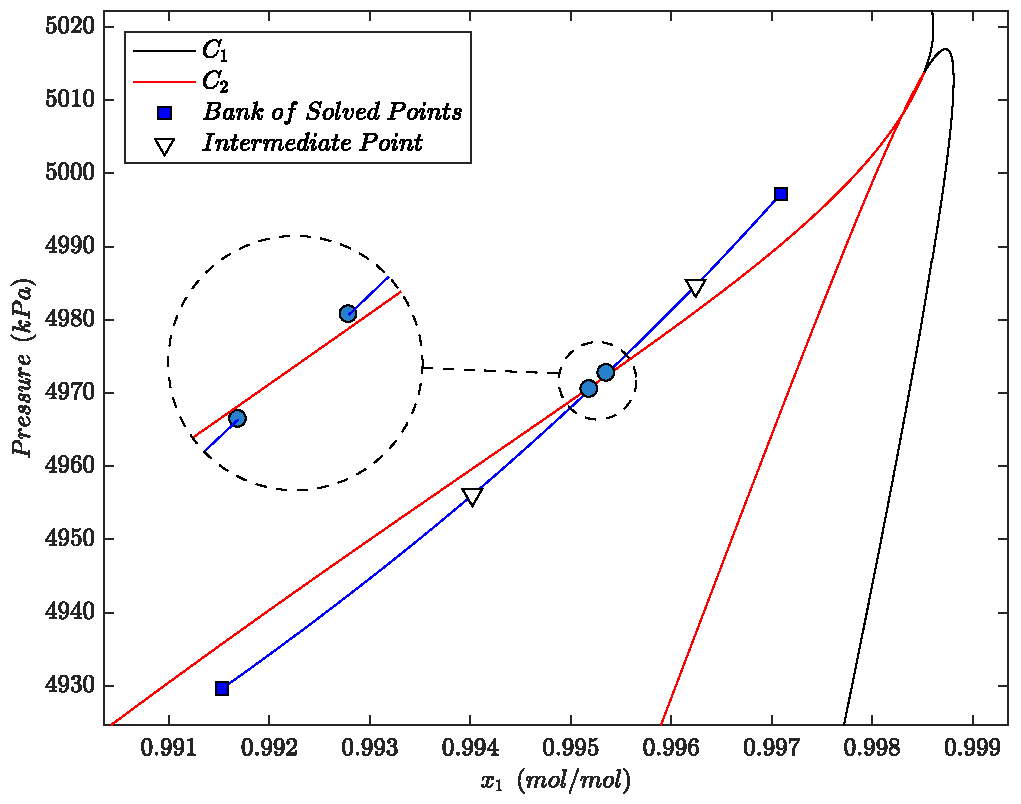
\includegraphics[scale=0.50]{caminhos_L_degeneracao_dominio_new.pdf}
		\caption{The ``L'' path in the domain, Roots 3 and 4.}\label{fig:L_path_domain}
	\end{center}
\end{figure}

%\subsubsection{Moving to the left}
%
%Another interesting possibility is to approach the critical image moving to the left. In this case, we do not observe the same behaviour when compared to the movement to the right portion of the figure. Only one pre-image approaches to the critical curve (in the domain), as detailed in Figures \ref{fig:image_left} and \ref{fig:domain_left}. Then, we can conclude that one root (Root 4, using the numbering accordingly to Table \ref{tab:roots}) will disappear. This fact is compatible to the physical reduction of the temperature of the system, where the ``double-dome'' structure (four dew points) vanishes in the transition to the S-type structure (three dew points). Furthermore, the distance $\delta$ in Figure \ref{fig:domain_left} tends to zero when the final of the critical curve $C_2$ is approached. 
%
%\begin{figure}
%	\begin{center}
%		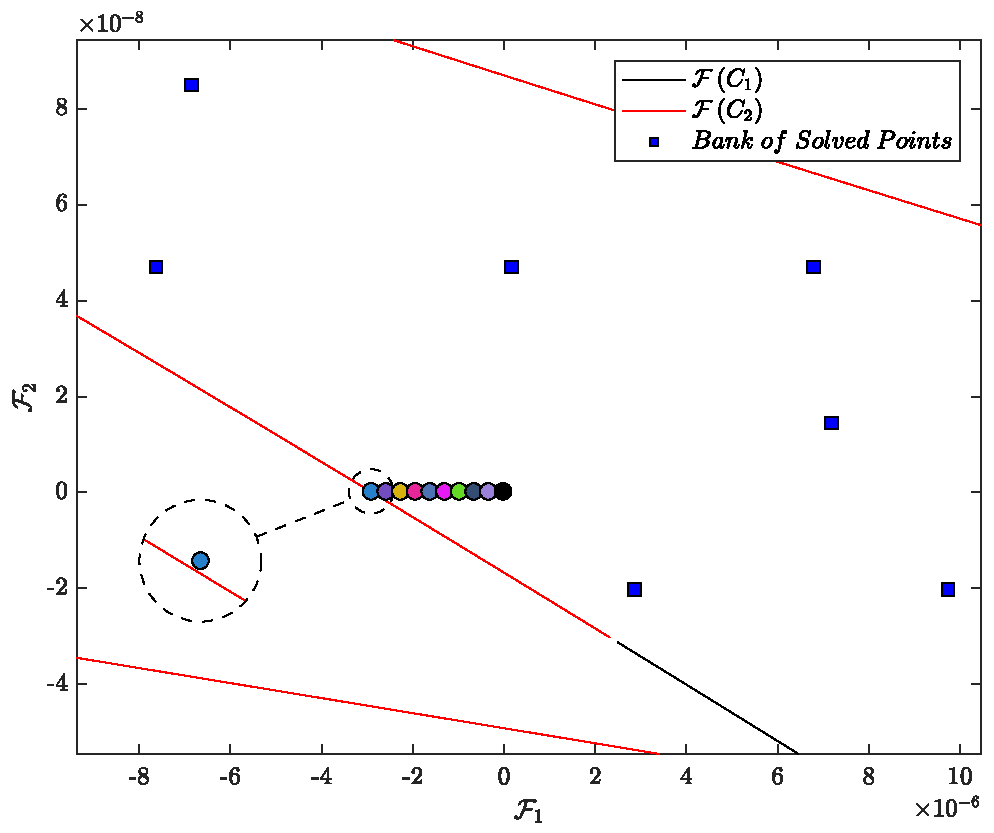
\includegraphics[scale=0.50]{imagem_new.pdf}
%		\caption{Sequence of inverted points (image).}\label{fig:image_left}
%	\end{center}
%\end{figure}
%
%\begin{figure}
%	\begin{center}
%		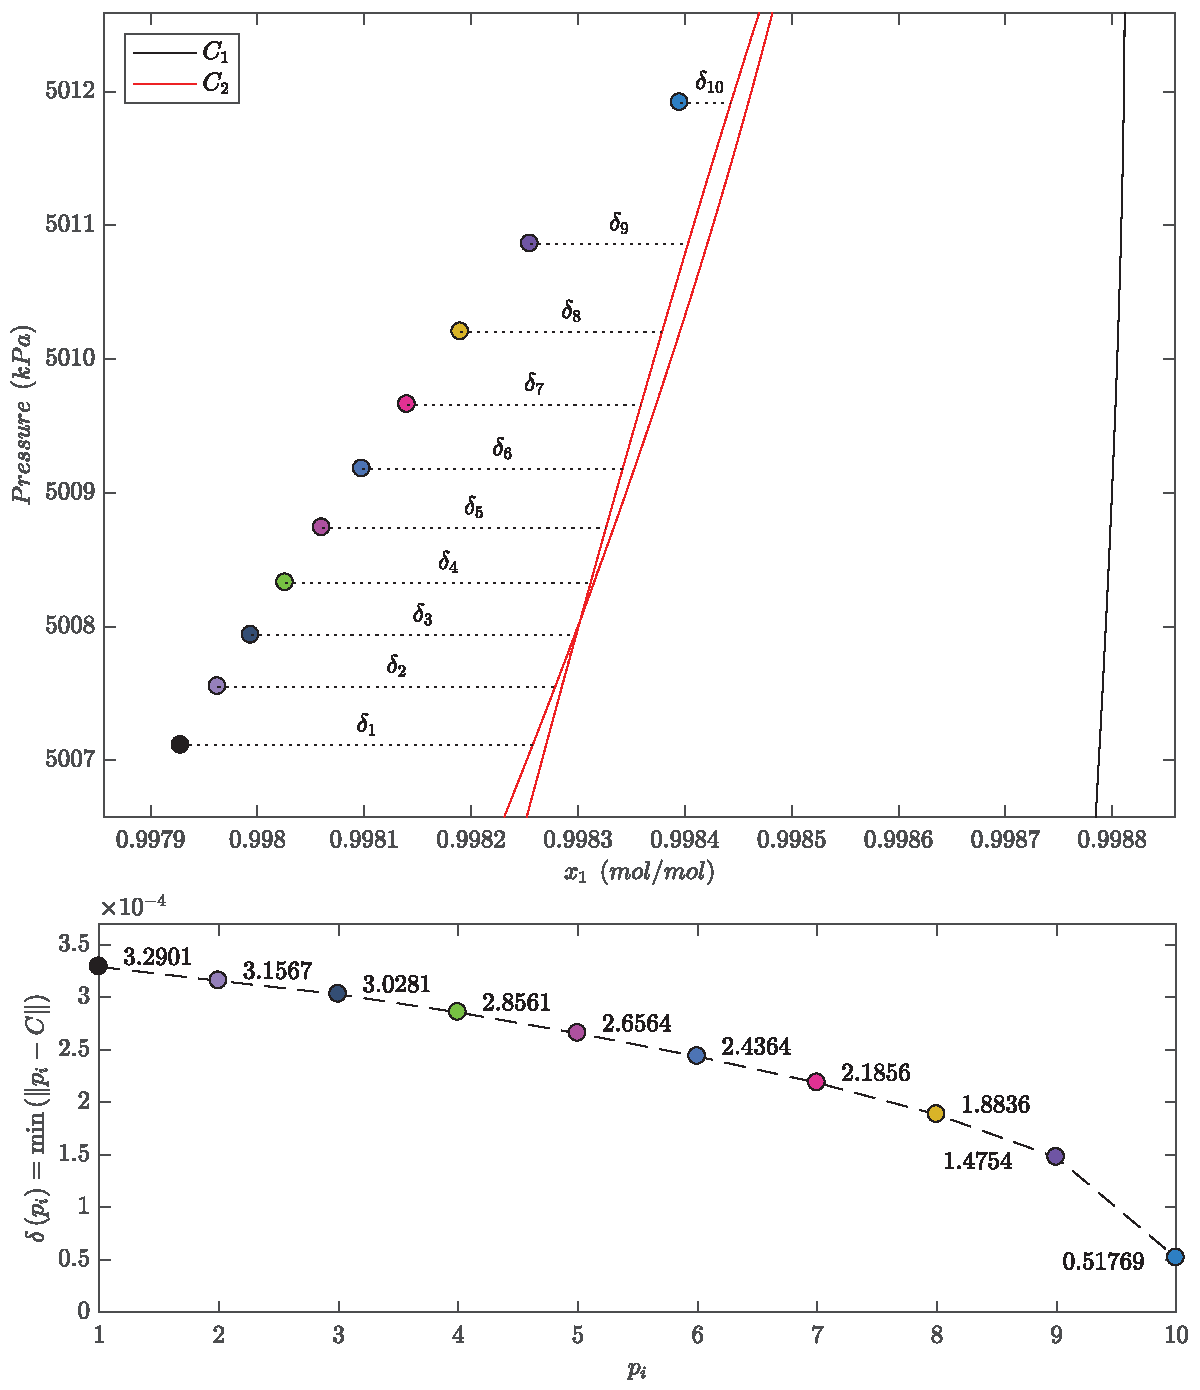
\includegraphics[scale=0.50]{dominio_distancias_new.pdf}
%		\caption{Sequence of inverted points (domain), Root 4.}\label{fig:domain_left}
%	\end{center}
%\end{figure}

\subsection{Results at $T$ = 304.5 K and $y_1 = 0.99945$}

At $T = 304.5$ K and $y_1 = 0.99945$, the dew point curve still exhibits a double retrograde behavior, but now as a ``S'' shape (instead of a double dome). In this situation, we observed three dew point pressures (and liquid compositions) for a narrow range of molar fractions.

Figure \ref{fig:imagem_S} shows the path of the inversion processes, beginning at $q = (0,0)$ and approaching to the critical image.

\subsubsection{Inversion Process -- Approaching to the critical image}

\begin{figure}
	\begin{center}
		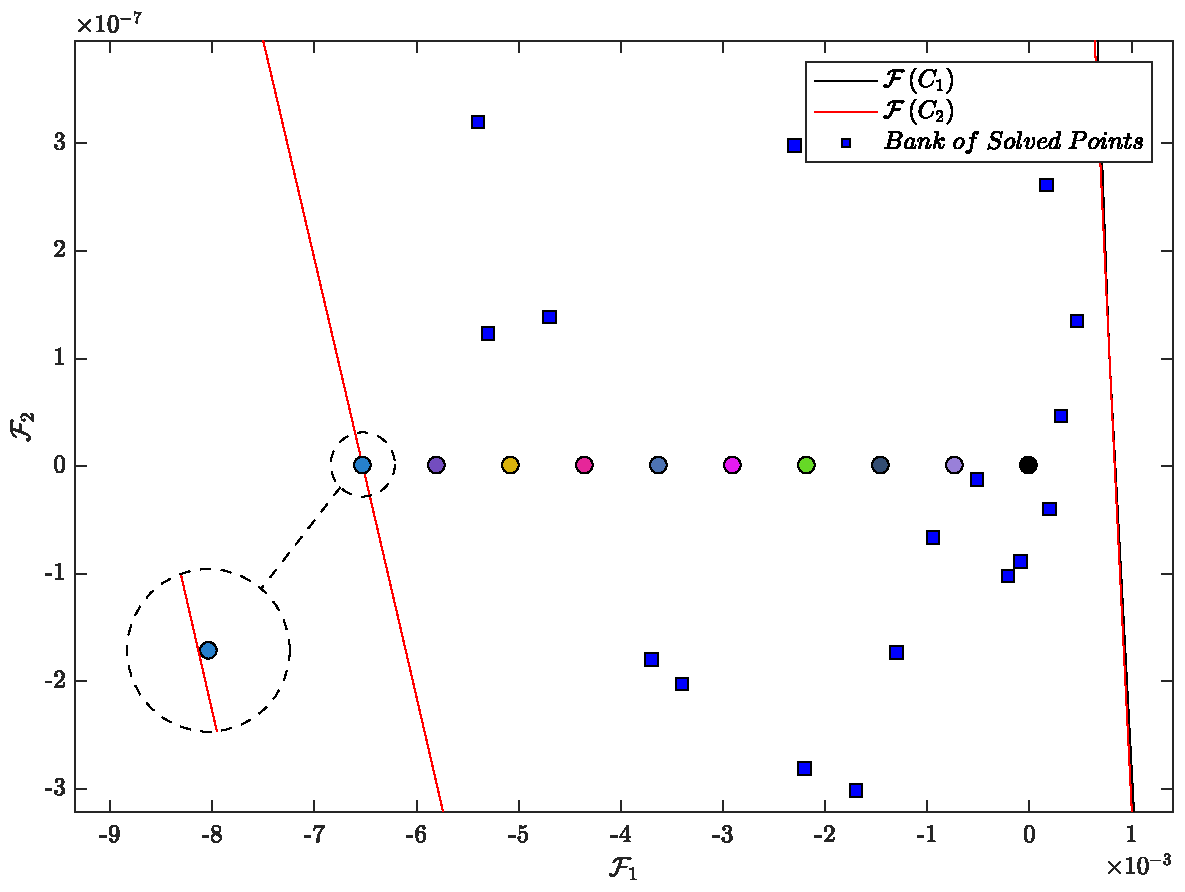
\includegraphics[scale=0.45]{imagem3.pdf}
		\caption{Sequence of inverted points (image) for $T$ = 304.5 K and $y_1 = 0.99945$.}\label{fig:imagem_S}
	\end{center}
\end{figure}

The movement of the pre-images obtained in the inversion process is illustrated in Figure \ref{fig:domain_S}. We noted that, when $q$ approaches to the critical image, two pre-images tend to disappear in a fold. We also displayed the kernel of the Jacobian matrix ($ker(J)$).


\begin{figure}
	\begin{center}
		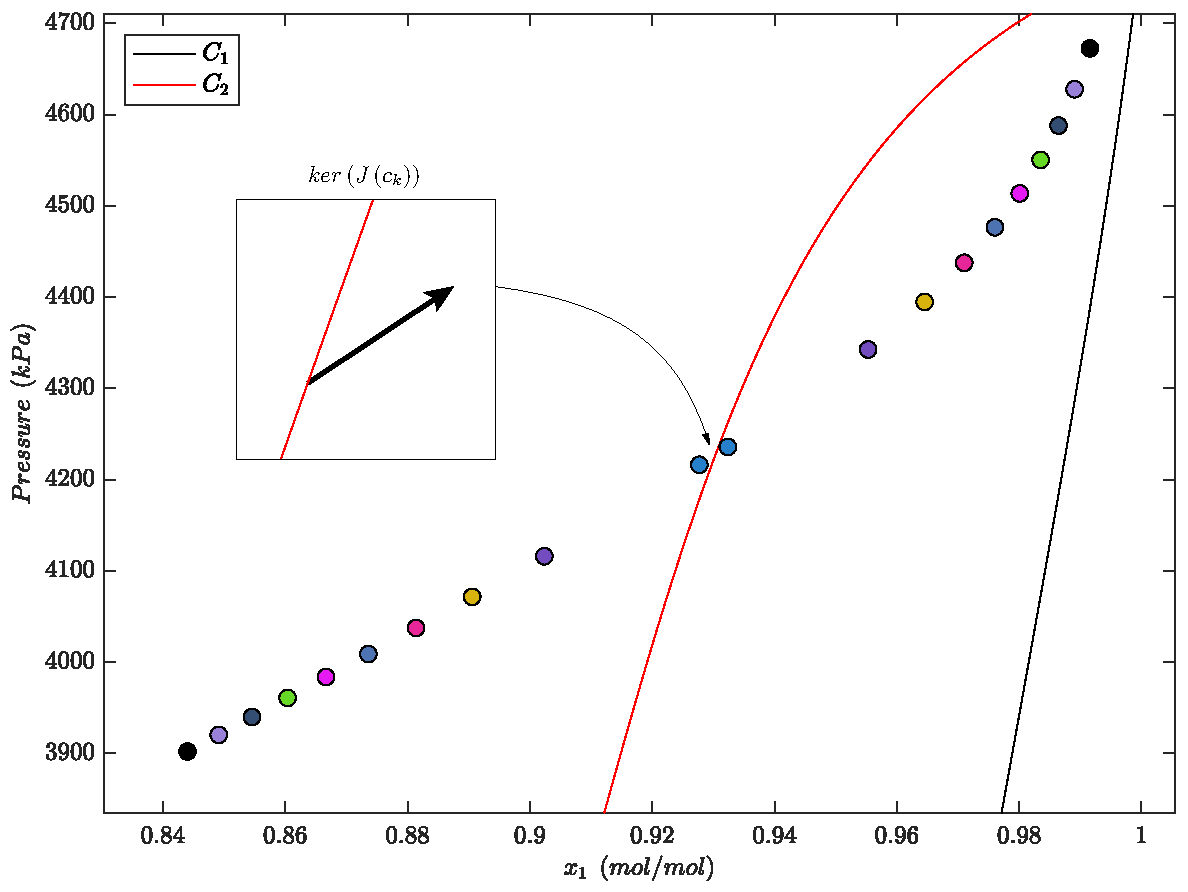
\includegraphics[scale=0.50]{dominio3.pdf}
		\caption{Sequence of inverted points (domain) for $T$ = 304.5 K and $y_1 = 0.99945$ (Roots 2 and 3).}\label{fig:domain_S}
	\end{center}
\end{figure}

Finally, Figure \ref{fig:L_S} illustrates the ``L'' path of the inversion process in domain for the last point (marked in blue in the two previous figures). Again, we can note the two pre-images corresponding to the Roots 2 and 3 tend to degenerate to a unique pre-image.

\begin{figure}
	\begin{center}
		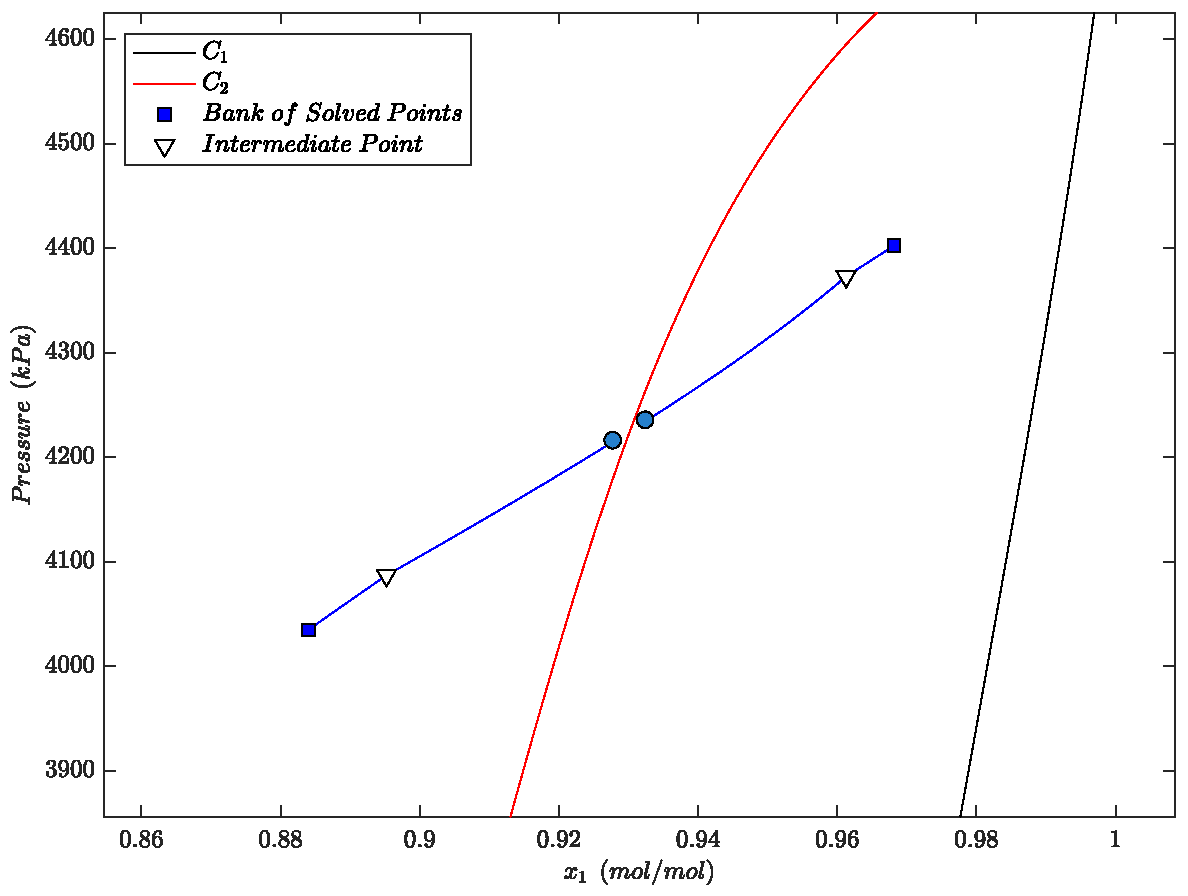
\includegraphics[scale=0.50]{caminhos_L_degeneracao_dominio2.pdf}
		\caption{The ``L'' path in the domain, Roots 2 and 3, for $T$ = 304.5 K and $y_1 = 0.99945$.}\label{fig:L_S}
	\end{center}
\end{figure}



\subsection{The influence of the temperature in the critical curve}

The last feature to be approached in this work corresponds to the influence of the system temperature (specified) in the critical curve. Obviously, the DRV phenomenon is a function of the temperature. 

\section{Conclusions}

% Bibliography
%-----------------------------------------------------------------
\begin{thebibliography}{99}

\bibitem{ireme} Libotte, G. B., Moura Neto, F. D., Guedes, A. L., Platt, G. M. (2016). Robust Prediction of Double Retrograde Vaporization
by Numerical Inversion of Functions, \emph{International Review of Mechanical Engineering (Testo Stampato)}, 10(6), 452-460.

\bibitem{canadian} Guedes, A. L., Moura Neto, F. D., Platt, G. M. (2015). Prediction of Azeotropic Behaviour by the Inversion of Functions from the Plane to the Plane, \emph{The Canadian Journal of Chemical Engineering}, 93, 914-928.

\bibitem{malta} Malta, I. P., Saldanha, N. C., Tomei, C. (1996). The Numerical Inversion of Functions from the Plane to the Plane, \emph{Mathematics of Computation}, 65(2016), 1531-1552.

\bibitem{classif} Van Konynenburg, P. H., Scott, R. L. (1980). Critical lines and phase equilibria in binary van der Waals mixtures, \emph{Phylosophical Transactions of The Royal Society of London A: Mathematical, Physical and Engineering Sciences}, 298(1442), 495-540.

\bibitem{heidemman} Heidemman, R. A., Khalil, A. M. (1980). The calculation of critical points, \emph{AIChE Journal}, 26(5), 769-779.

\bibitem{peng_robinson} Peng, D., Robinson, D. (1976). A new two-constant equation of state, \emph{Industrial \& Engineering Chemistry Research}, 15(1), 59-64.

\bibitem{raeissi_1} Raeissi, S., Peters, C. J. (2001). On the phenomena of double retrograde vaporization: multi dew point behavior in the binary system ethane + limonene, \emph{Fluid Phase Equilibria}, 191, 33-40.

\bibitem{raeissi_2} Raeissi, S., Peters, C. J. (2001). Simulation of double retrograde
vaporization using the Peng-Robinson equation of state, \emph{Journal of Chemical Thermodynamics}, 35, 573-581.

\bibitem{chen_1} Chen, R. J. J., Chappelear, P. S., Kobayashi, R. (1974). Dew point loci for methane-n-butane binary system, \emph{Journal of Chemical and Engineering Data}, 19, 53-58.

\bibitem{chen_2} Chen, R. J. J., Chappelear, P. S., Kobayashi, R. (1974). Dew point loci for methane-n-pentane binary system, \emph{Journal of Chemical and Engineering Data}, 19, 59-61.

\bibitem{jnsa} Platt, G. M., Bastos, I. N., Domingos R. P. (2012). Calculation of double retrograde vaporization: Newton's methods and Hyperheuristic approach, \emph{Journal of Nonlinear Systems and Applications}, 3(2), 107-120.

\end{thebibliography}

\end{document}
